\documentclass[usenatbib]{latex/mn2e} 
%External Packages and personalized macros
%=========================================================================
%		EXTERNAL PACKAGES
%=========================================================================
\usepackage{amsmath} 
\usepackage{amssymb} 
\usepackage {graphicx}
%\usepackage{graphics}
\usepackage[dvips]{epsfig}
\usepackage{epsfig}  
\usepackage{color}
\usepackage[normalem]{ulem}
\usepackage{hyperref}
\usepackage{caption}

%=========================================================================
%		INTERNAL MACROS
%=========================================================================
\def\be{\begin{equation}}
\def\ee{\end{equation}}
\def\ba{\begin{eqnarray}}
\def\ea{\end{eqnarray}}

% To highlight comments 
\definecolor{red}{rgb}{1,0.0,0.0}
\newcommand{\red}{\color{red}}
\definecolor{darkgreen}{rgb}{0.0,0.5,0.0}
\newcommand{\SRK}[1]{\textcolor{darkgreen}{\bf SRK: \textit{#1}}}
\newcommand{\SRKED}[1]{\textcolor{darkgreen}{\bf #1}}

\newcommand{\LCDM}{$\Lambda$CDM~}
\newcommand{\beq}{\begin{eqnarray}}  
\newcommand{\eeq}{\end{eqnarray}}  
\newcommand{\zz}{$z\sim 3$} 
\newcommand{\apj}{ApJ}  
\newcommand{\apjs}{ApJS}  
\newcommand{\apjl}{ApJL}  
\newcommand{\aj}{AJ}  
\newcommand{\mnras}{MNRAS}  
\newcommand{\mnrassub}{MNRAS accepted}  
\newcommand{\aap}{A\&A}  
\newcommand{\aaps}{A\&AS}  
\newcommand{\araa}{ARA\&A}  
\newcommand{\nat}{Nature}  
\newcommand{\physrep}{PhR}
\newcommand{\pasp}{PASP}    
\newcommand{\pasj}{PASJ}    
\newcommand{\avg}[1]{\langle{#1}\rangle}  
\newcommand{\ly}{{\ifmmode{{\rm Ly}\alpha}\else{Ly$\alpha$}\fi}}
\newcommand{\hMpc}{{\ifmmode{h^{-1}{\rm Mpc}}\else{$h^{-1}$Mpc }\fi}}  
\newcommand{\hGpc}{{\ifmmode{h^{-1}{\rm Gpc}}\else{$h^{-1}$Gpc }\fi}}  
\newcommand{\hmpc}{{\ifmmode{h^{-1}{\rm Mpc}}\else{$h^{-1}$Mpc }\fi}}  
\newcommand{\hkpc}{{\ifmmode{h^{-1}{\rm kpc}}\else{$h^{-1}$kpc }\fi}}  
\newcommand{\hMsun}{{\ifmmode{h^{-1}{\rm {M_{\odot}}}}\else{$h^{-1}{\rm{M_{\odot}}}$}\fi}}  
\newcommand{\hmsun}{{\ifmmode{h^{-1}{\rm {M_{\odot}}}}\else{$h^{-1}{\rm{M_{\odot}}}$}\fi}}  
\newcommand{\Msun}{{\ifmmode{{\rm {M_{\odot}}}}\else{${\rm{M_{\odot}}}$}\fi}}  
\newcommand{\msun}{{\ifmmode{{\rm {M_{\odot}}}}\else{${\rm{M_{\odot}}}$}\fi}}  
\newcommand{\lya}{{Lyman$\alpha$~}}
\newcommand{\clara}{{\texttt{CLARA}}~}
\newcommand{\rand}{{\ifmmode{{\mathcal{R}}}\else{${\mathcal{R}}$ }\fi}}  

%MY COMMANDS #############################################################
\newcommand{\sub}[1]{\mbox{\scriptsize{#1}}}
\newcommand{\dtot}[2]{ \frac{ d #1 }{d #2} }
\newcommand{\dpar}[2]{ \frac{ \partial #1 }{\partial #2} }
\newcommand{\pr}[1]{ \left( #1 \right) }
\newcommand{\corc}[1]{ \left[ #1 \right] }
\newcommand{\lla}[1]{ \left\{ #1 \right\} }
\newcommand{\bds}[1]{\boldsymbol{ #1 }}
\newcommand{\oiint}{\displaystyle\bigcirc\!\!\!\!\!\!\!\!\int\!\!\!\!\!\int}
\newcommand{\mathsize}[2]{\mbox{\fontsize{#1}{#1}\selectfont $#2$}}
\newcommand{\eq}[2]{\begin{equation} \label{eq:#1} #2 \end{equation}}
%#########################################################################

\begin{document}

%=========================================================================
%		FRONT MATTER
%=========================================================================
\title[LG Environment]{The place of the local group in the cosmic web}
\author[S. Bustamante and J.E. Forero-Romero]{
\parbox[t]{\textwidth}{\raggedright 
  Sebastian Bustamante \thanks{sbustama@pegasus.udea.edu.co}$^{1}$ 
  Jaime E. Forero-Romero$^{2}$ 
}
\vspace*{6pt}\\
$^1$Instituto de F\'{\i}sica - FCEN, Universidad de Antioquia, Calle
67 No. 53-108, Medell\'{\i}n, Colombia\\ 
$^2$Departamento de F\'{i}sica, Universidad de los Andes, Cra. 1
No. 18A-10, Edificio Ip, Bogot\'a, Colombia
}

\maketitle

\begin{abstract}


We present a theoretical study Local Group in a cosmological context. 

The principal objective is to find a coherent  
sample of LG systems in the unconstrained simulation Bolshoi based upon 
the properties of hand construted LG systems in the constrained 
simulations CLUES. We obtain a privileged environment for these systems 
and significant bias in some of their properties. (\SRKED{draft!})


\end{abstract}

\begin{keywords}
galaxies: high-redshift - galaxies: star formation - line: formation
\end{keywords}


%=========================================================================
%		PAPER CONTENT
%=========================================================================

%*************************************************************************
\section{Introduction}
\label{sec:introduction}
%*************************************************************************


The spatial distribution of galaxies describes a web-like pattern, the 
so-called cosmic web. Today it is understood that such configuration
is driven by gravitational instabilities. ...

The study of the influence of the cosmic web on galaxy properties
start with the seminal work of Dressler \SRKED{[reference here]} and
extends to recent works using large observational surveys that look
for signatures of the web into the evolution of galaxy
populations. With the advention of more detailed observations and
sophisticated computational models it is now within our reach to
understand what physical processes dominate.

This makes  that the mass
assembly history of a galaxy is deeply connected with its  position in
the cosmic web. There is an extensive body of literature on  the
effects of the web environment on the observable properties of
galaxies. 


This environmental study is also of paramount importance to understand
the formation of our Galaxy. In our local neighborhood, the
observations of dwarf galaxies around the Milky Way (MW) and the
Andromeda galaxy (M31) show filamentary and disk-like patterns that
can be linked to a preferential infall direction, very likely
connected with the cosmic web where the Local Group (LG) of galaxies
is embedded. 

In this paper we quantify the velocity shear environment of DM halo pairs
representative of the principal members of the Local Group (LG), the Milky 
Way (MW) and Andromeda galaxy (M31). We perform this study in two kinds of 
cosmological simulations: unconstrained simulations from random phases in 
the initial conditions, together with constrained simulations, which have 
been setup as to reproduce the large scale structure of the local universe
($\sim 30$\hMpc around the local group) on scales of $\sim 5$\hMpc. 


We pay special attention to the correlation of the present velocity shear 
environment with the assembly and the kinematics properties of the pairs. 
The motivation to have that focus is that it has been previously shown that 
the LG present in three different realizations of the constrained simulations 
have assembly histories biased towards early formation times and absence of 
major mergers (ratio 1:10) in the last $10$ Gyr. In the case of the kinematic
properties, recent observational constrains to the galactocentric tangential 
velocity of M31 has enabled to establish how typical is the LG in a 
cosmological context \SRKED{[reference to Forero-Romero 2013-1]}, that is why
we focus here how a specific kind of host environment biases these kinematics
properties.


%*************************************************************************
\section{The Simulations}
\label{sec:the_simulations}
%*************************************************************************


We use two sets of simulations two identify the possible large scale 
environment of the Local Group. This is similar approach to the one 
already used by \SRKED{[reference here]}. The first set of simulations are 
constrained, that aim at reproducing the large scale environment around the 
local group as described by observations. The second simulations is an 
unconstrained cosmological volume that serve us as a benchmark of the results 
obtained from the constrained realizations. In the following subsections we 
describe the most relevant characteristics of these two simulations.


%-------------------------------------------------------------------------
\subsection{The CLUES simulations}
\label{subsec:CLUES_simulations}
%-------------------------------------------------------------------------


The CLUES simulations have constrained initial conditions. The design goal 
was being able to reproduce in a N-body simulation the density distribution 
in the local universe on scales of $\sim5$ Mpc as accurate as the 
observations allow. A full description of the methods and results in the 
CLUES project was done by \SRKED{[reference here]}, a summary  of the 
cosmological volumes we use in this paper was presented by 
\SRKED{Forero-Romero et al. 2011.}


The most relevant technical details are the following. We use three DM only
simulations done in cubic volumes of $64$\hMpc (comoving) on a side. The 
matter field is sampled with $1024^3$ particles, the integration was 
performed using the Tree-PM MPI N-body code Gadget2 \SRKED{[reference here]}. 
The cosmological parameters are consistent with a WMAP5 and WMAP7 cosmologies 
with $\Omega_{\rm m}=0.28$, $\Omega_{\Lambda}=0.72$, $h=0.73$, $n=0.73$ and 
$\sigma_{8}=0.817$ \SRKED{[reference to Komatsu]} for the matter density, 
cosmological constant, dimensionless Hubble parameter, spectral index of 
primordial density perturbations and normalization for the power spectrum. 
With these parameters the mass of each particle in the simulation is 
$m_{\rm p}=1.89\times 10^{7}$\hMsun.


%-------------------------------------------------------------------------
\subsection{The Bolshoi simulation}
\label{subsec:Bolshoi_simulation}
%-------------------------------------------------------------------------

The Bolshoi simulations follows the non-linear evolution of a dark
matter density field on a cubic volume of size $250$\hMpc
sampled with $2048^3$ particles. The cosmological parameters in the
simulation are $\Omega_{\rm m}=0.27$, $\Omega_{\Lambda}=0.73$,
$h=0.70$, $n=0.95$ and $\sigma_{8}=0.82$ for the matter density, 
cosmological constant, dimensionless Hubble parameter, spectral index
of primordial density perturbations and normalization for the power
spectrum. The mass of each particle in the simulation is $m_{\rm
  p}=1.4\times 10^{8}$\hMsun.




%-------------------------------------------------------------------------
\subsection{Halos and Merger Trees}
\label{subsec:halos_merger_trees}
%-------------------------------------------------------------------------

We identify halos with a Friends-of-Friends (REF) algorithm. These 
catalogues also provide the basis for the mass aggregation history studies. 
All the results presented here must be interpreted in term of host halos, 
without any information of the substructure. In particular the merger of 
two FOF halos corresponds to the epoch of first overlap, and not to the 
fusion and/or disruption of an accreted sub-halo with a dominant halo. 


The linking length is $b=0.17$ times the mean inter-particle 
separation. All objects with 20 particles or more are considered a bona 
fide halo and are included in the construction of the merger tree, this 
corresponds to a minimum halo mass of $M_{\rm min}=3.78\times 10^{8}$
\hMsun in the CLUES volumes and $M_{\rm min}=2.70\times 10^{9}$\hMsun in 
the Bolshoi simulation. 


The halo identification for the CLUES simulation was done for 80
snapshots in the redshift range $0<z<7$ more or less evenly spaced in
look-back time. For Bolshoi we use the information of XX snapshots in
the same redshift range.


%*************************************************************************

\section{Algorithms to find the cosmic web}

\subsection{The tidal web - T-web}
The first algorithm  we use to identify the cosmic web is based on the
diagonalization of the tidal tensor, defined as the Hessian of a
normalized gravitational potential  

\begin{equation}
T_{\alpha\beta} = \frac{\partial^2\phi}{\partial x_{\alpha}\partial x_{\beta}}
\end{equation}

where the physical gravitational potential has been rescaled by a factor $4\pi
G\bar{\rho}$ in such a way that $\phi$ satisfies the folowing equation

\begin{equation}
\nabla^2\phi = \delta,
\end{equation}
 where $\bar{\rho}$ is the average density in the
Universe, $G$ is the gravitational constant and $\delta$ is the
dimensionless matter overdensity.

\subsection{The velocity  web - V-web}
\label{sec:Vweb}
%*************************************************************************


We use the a kinematical method to define the cosmic-web environment in 
the simulation. The method has been thoroughly described in XXX and 
applied to study the shape and spin alignment in the Bolshoi simulation 
here XX. We refer the reader to these papers to find a detailed description 
of the algorithm, its limitations and capabilities. Here we summarize the
most relevant points for the discussion. 


The V-web method for environment finding is based on the local shear 
tensor calculated from the smoothed DM velocity field in the simulation.
The central quantity is the following dimensionless quantity 


%.........................................................................
%V-Web Definition
\eq{V_web}
{
\Sigma_{\alpha\beta} = -\frac{1}{2H_0}\pr{\frac{\partial v_{\alpha}}
{\partial x_{\beta}}+\frac{\partial v_{\beta}}{\partial x_{\alpha}}}
}
%.........................................................................
where $v_{\alpha}$ and $x_{\alpha}$ represent the $\alpha$ component of 
the comoving velocity and position, respectively. $\Sigma_{\alpha\beta}$ 
can be represented by a $3\times 3$ symmetric matrix with real values, 
that ensures that is possible to diagonalize and obtain three real 
eigenvalues $\lambda_{1} > \lambda_{2}>\lambda_3$ whose sum (the trace of
$\Sigma_{\alpha\beta}$) is proportional to the divergence of the local 
velocity field smoothed on the physical scale ${\mathcal R}$. 


The relative strength of the three eigenvalues with respect to a threshold
values $\lambda_{th}$ allows for the local classification of the matter 
distribution into four web types. Voids, sheets, filaments and peaks, 
which correspond to regions with 3, 2, 1 or 0 eigenvalues with values 
larger than $\lambda_{th}$. In this paper we do not perform an definitive 
classification into web types, instead we express the results respect to 
the relative strength of the eigenvalues and in a range of $\lambda_{th}$.
To choose a suitable range we propose a new quantity analogous to 
expression \ref{eq:V_web}, but built with the physical velocity field 
$w_{\alpha}$ and physical coordinates $r_{\alpha}$, the physical local 
shear tensor, defined as 


%.........................................................................
%Physical V-Web
\eq{V_web_Phys}
{
\Pi_{\alpha\beta} = -\frac{1}{2H}\pr{\frac{\partial w_{\alpha}}
{\partial r_{\beta}}+\frac{\partial w_{\beta}}{\partial r_{\alpha}}}
}
%.........................................................................
evaluating this quantity in current epoch, we obtain the next relation 
between both tensors


%.........................................................................
%Relation between V-web tensors
\eq{Rel_Tensors}
{ \Pi_{\alpha\beta} = \Sigma_{\alpha\beta} - \delta_{\alpha\beta} }
%.........................................................................


Using this relations, we can establish the two extreme $\lambda_{th}$ 
values to present our results. The first one $\lambda_{th} = 0$, it is 
obtained assuming that the sign of each eigenvalue indicates the nature of
collapse in the respective direction, what is valid in the strong 
non-linear scale where the peculiar velocity field is mainly dominant. 
The upper limit $\lambda_{th} = 1$ is obtained using the same previous 
argument, but using the eigenvalues of the the physical tensor, what is 
valid in the weak non-linear scale, where the hubble flow is still 
dominant.


We consider \textit{a posteriori} the possible web type interpretation 
that could be feasible within a range of thresholds for the eigenvalues. 


\subsection{The Web in Bolshoi and CLUES}
... Resolution and Smoothing

... Database

%*************************************************************************
\section{Local Group Sample Definition}
\label{section:Def_Samples}
%*************************************************************************


We define list here conditions that have to fulfill a pair of halos in a 
unconstrained simulation to be considered as LG-like. All considerations 
are based on the relative dynamics of the Milky Way and M31, and its 
isolation from massive structures:


%.........................................................................
%Isolated pairs criteria
\begin{enumerate}
\item{The Local Group is considered to be a pair of halos with dark matter 
masses in the range $5\times10^{11}<M_{h}/\hMsun < 5\times 10^{12}$.}

\item{The distance between the center of the two halos should be less than 
$0.7$\hMpc.}

\item{The relative physical velocity between the two halos has to be 
negative.}

\item{The distance to any halo more massive than any of the pair members 
must be less than $XX$\hMpc.}

\item{The distance to cluster-like halos with masses larger than $XX$\hMpc 
must be larger than $XX$\hMpc.}
\end{enumerate}
%.........................................................................


In the case of a constrained simulation on can include an additional 
constrain


%.........................................................................
%Additional criteria
\begin{enumerate}
\item[(vi)]{The Local Group pair must be located in the right environment 
with respect to the XX Cluster.}
\end{enumerate}
%.........................................................................


From these conditions it is possible to construct three different samples.
A sample of pairs, following conditions 1 to 3. A second sample of 
isolated pairs, that additionally fulfill conditions 4 and 5, and a sample 
third sample of LGs that fulfills condition 6. The samples of pairs and 
isolated pairs can be constructed from the Bolshoi and CLUES simulations. 
However, by construction, the LGs sample can only be extracted from the 
constrained simulation.


%.........................................................................
%Table of samples numbers
\begin{table}
  \centering
  \begin{tabular}{l | c c c c} \hline
	\textbf{Sample}& \textbf{CLUES} & \textbf{CLUES} & \textbf{CLUES} & \textbf{Bolshoi} \\
	\textbf{description}& \textbf{2710} & \textbf{10909} & \textbf{16953} &  \\ \hline
	General halos 	& 56632 & 57707 & 56799  & 432000 	\\
	Pairs 			& 386 	& 380 	& 387	 & 23037 	\\
	Isolated pairs	& 20 	& 12 	& 18 	 & 1256 	\\
	LG 				& 1 	& 1 	& 1 	 & 17		\\ \hline
  \end{tabular}
  
  \caption{Samples size in each simulation used. The relation between size 
  of samples in each CLUES simulations and Bolshoi is approximately $4^3$, 
  according to their volumes relation. ?? }
  
  \label{Tab:Samples}
\end{table}
%.........................................................................


%*************************************************************************
\section{Finding a Local Group environment}
\label{sec:experiments}
%*************************************************************************


In this section we prepare some numerical experiments with the halos 
samples and their environment, with special emphasis on the isolated pairs 
and LG samples. All this in order to find for environment correlations and 
common properties between LG systems.


%-------------------------------------------------------------------------
\subsection{Comparison of the two simulations}
\label{subsec:comparison_simulations}
%-------------------------------------------------------------------------


Prior to study of isolated and LG samples and to determinate possible 
correlations between their properties, it is necessary to establish the 
equivalence between all simulations that we will use, with the aim to 
eliminate effects due to construction process of each one.


In first place, we analyse the mass distribution of individual halos and 
in next figure we show the integrated mass function (IMF) for halos sample
with $M \geq 1\times 10^{11} M_{\odot}$.


%.........................................................................
%IMF halos
\begin{flushleft}
\begin{center}

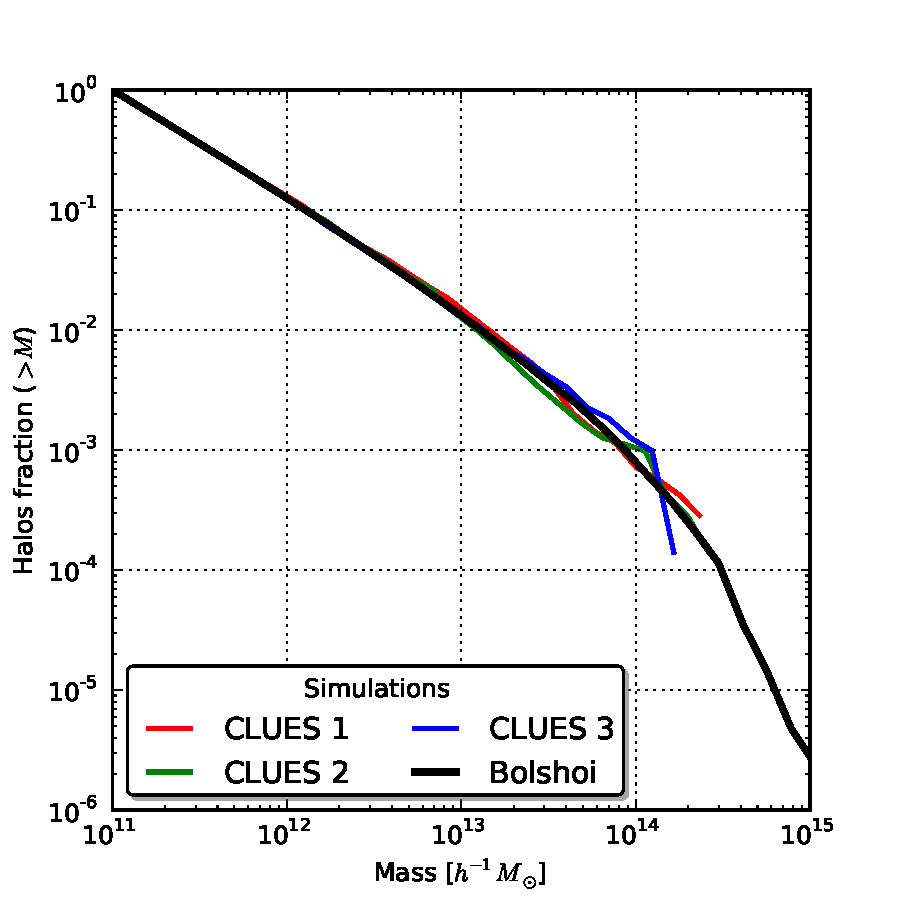
\includegraphics[keepaspectratio=true,width=0.35\textheight]
{./figures/Halos_IMF.pdf}

\captionof{figure}{\small Integrated mass function of individual halos of 
each simulation used. In the center-left, with vertical dot lines, the 
individual masses of each LG system in CLUES simulations are represented.}

\label{fig:IMF_Halos}
\vspace{0.1 cm}
\end{center}
\end{flushleft}
%.........................................................................


Although in high masses the IMF of each simulation are slightly different, 
in low mass region, where the most halos of our interest are, the IMFs are 
quite similar indicating that the sample of halos in each simulation have 
the same mass distribution, while the small differences are due to finite 
size of samples. Another aspect in the figure \ref{fig:IMF_Halos} is the 
position of LG halos, they are distributed across the mass range of halos 
that we have set (see in section \ref{section:Def_Samples}), indicating 
that there is not an apparent condition with their individual masses.


%.........................................................................
%Index Pairs
\begin{flushleft}
\begin{center}

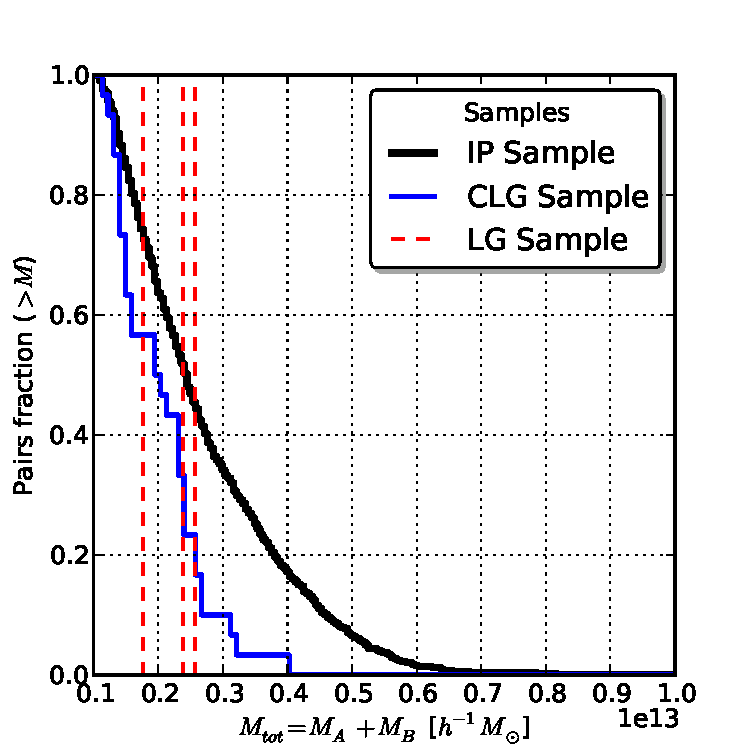
\includegraphics[keepaspectratio=true,width=0.3\textheight]
{./figures/IP_IMF.pdf}
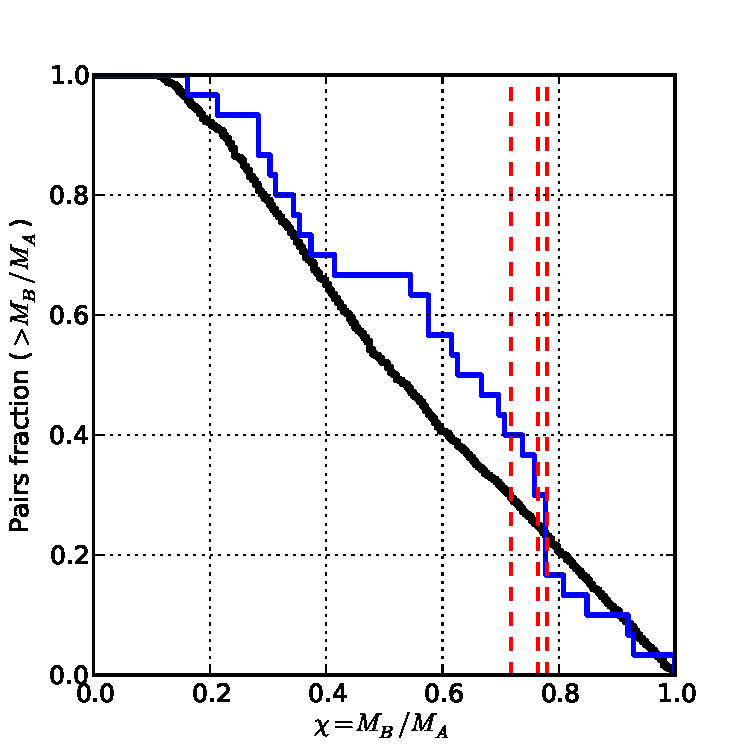
\includegraphics[keepaspectratio=true,width=0.3\textheight]
{./figures/IP_Mass_Ratio.pdf}

\captionof{figure}{\small Integrated distribution of mass ratio index for 
isolated pairs sample (a).}

\label{fig:Index_Pairs}
\vspace{0.1 cm}
\end{center}
\end{flushleft}
%.........................................................................


The situation is quite different respect to mass ratio index of isolated 
pairs sample (MRI). In the figure \ref{fig:Index_Pairs} (a) we show the 
integrated distribution of MRI, where the approximately linear behaviour 
indicates an uniformly distribution. The interesting aspect here is the 
closeness between the LG sample values, indicating a possible common 
property in these systems, even though this could be established a priori 
by construction. In the \ref{fig:Index_Pairs} (b) is plotted the 
integrated distribution of total pair mass, and again like the IMF, there 
is not a preferential value.


Once established the concordance between the defined samples, we proceed 
to analyse the distribution of the eigenvalue of shear velocity tensor 
\ref{eq:V_web}, for this we assume that the halos are good tracers of the 
environment properties and therefore we evaluate each eigenvalue in the 
center mass of each halo, mapping of this way the complete distribution 
(figure \ref{fig:lambda_histogram}). The black curves correspond to the 
unconstrained simulation (Bolshoi) and the color curves to the constrained 
simulations (CLUES), aditionally we calculate the cosmic variance, showed 
in purple curves, dividing the Bolshoi volume in smaller parts with a size 
comparable to the CLUES volume ($64 h^{-1 }$ Mpc of side). What is 
interesting here is the clear difference between the eigenvalues 
distributions of the both types of simulations, inclusively the 
constrained distributions does not match between the cosmic variance, 
indicating that although both simulations were made with the same cosmology 
(see subsections \ref{subsec:CLUES_simulations} and 
\ref{subsec:Bolshoi_simulation}), the constrained simulations have a 
significantly different environment properties (spatial matter distribution) 
compared to the average expected from a random volume with the same 
comoving size.


%.........................................................................
% Lambda Histogram
\begin{figure*}
\begin{center}
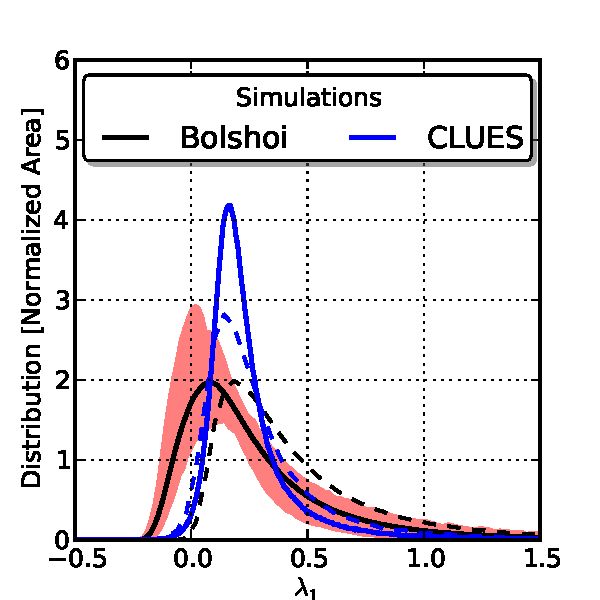
\includegraphics[trim = 0mm 0mm 5mm 8mm, clip, keepaspectratio=true,
width=0.24\textheight]{./figures/Cells_Distro_L1.pdf}
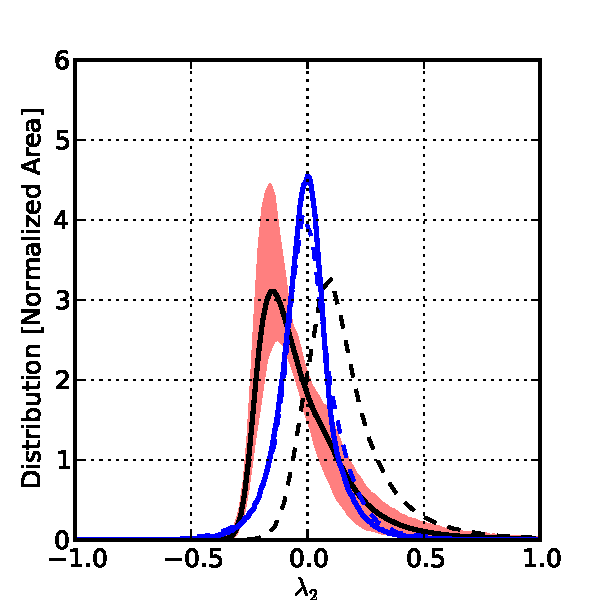
\includegraphics[trim = 0mm 0mm 5mm 8mm, clip, keepaspectratio=true,
width=0.24\textheight]{./figures/Cells_Distro_L2.pdf}
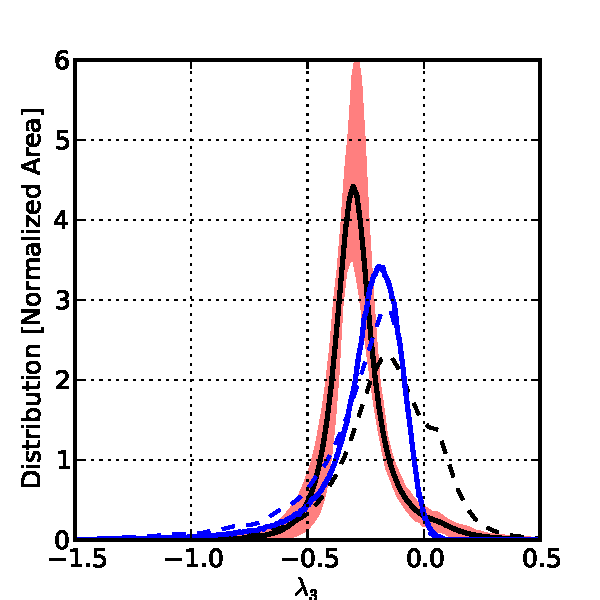
\includegraphics[trim = 0mm 0mm 5mm 8mm, clip, keepaspectratio=true,
width=0.24\textheight]{./figures/Cells_Distro_L3.pdf}

\caption{\small Integrated distribution of mass ratio index for isolated 
pairs sample (a).}

\label{fig:lambda_histogram}

\vspace{0.1 cm}
\end{center}
\end{figure*}
%.........................................................................


%-------------------------------------------------------------------------
\subsection{Defining the LG environment}
\label{subsec:LG_construction}
%-------------------------------------------------------------------------


With the aim of constructing a sample of LG systems in Bolshoi simulations, 
we use the eigenvalues of the three LG systems in each CLUES simulation 
and choose a range for each one based in the extreme values of the six 
halos, this with the expectation of reproducing the LG specific conditions 
in constrained simulations. This criteria can be thought as a first 
approximation to establish a more faithful sub-sample into the isolated 
pairs. In table \ref{Tab:Lambdas_LG} we show the used extreme values for 
each eigenvalue of local shear tensor.


%.........................................................................
%Table of extreme values of LG environment
\begin{table}
  \centering
  \begin{tabular}{l | c c c} \hline
	& $\bds{\lambda_{1}}$ & $\bds{\lambda_{2}}$  & $\bds{\lambda_{3}}$ \\ \hline
	\textbf{Minim value} & 1.77$\times 10^{-1}$ & -6.29$\times 10^{-3}$ & -1.98$\times 10^{-1}$ \\
	\textbf{Maxim value} & 3.49$\times 10^{-1}$ & 1.21$\times 10^{-1}$ & -8.85$\times 10^{-2}$ \\ \hline
  \end{tabular}
  
  \caption{Extreme values for each eigenvalues to construct LG samples.}
  
  \label{Tab:Lambdas_LG}
\end{table}
%.........................................................................


As a self-consistency test, we apply this criteria to CLUES simulations 
and find, on average, three LG systems in each one. But to avoid confusion, 
we keep defining the LG sample as the three initial pairs. Finally, we 
construct the LG sample of Bolshoi, where the sample size is illustrated 
in Table \ref{Tab:Samples}.


%-------------------------------------------------------------------------
%\subsection{Environment characterization}
%\label{subsec:Env_characterization}
%-------------------------------------------------------------------------


Once we have established the equivalence of samples in each simulation and 
have defined the LG samples, we proceed to calculate correlations between 
halo samples and their environment. As was mentioned in section 
\ref{sec:Vweb}, we do not use an specific value of eigenvalue threshold 
$\lambda_{th}$, instead of this, we explore a relatively wide range of 
this parameter (i.e. $0 \leq \lambda_{th} \leq 1$) and calculate 
distributions respect to each eigenvalue individually.


At first place, we calculate the environment of each LG system in CLUES 
simulations, for this we use the $\lambda_{th}$ scheme to classify it in 
void, sheet, filament or knot (see \ref{sec:Vweb}), with $\lambda_{th}$
into the threshold range. Figure \ref{fig:LG_Env_CLUES} is obtained.


At first place, we calculate the integrated distribution of each 
eigenvalue for individual halos, isolated pairs and LG samples. For this, 
we associate to each halo a value of environment (set of eigenvalues)
according to its center of mass position in a smoothed grid ($256^3$ 
cells for Bolshoi and $64^3$ for CLUES, or equivalently a resolution of 
$1.0 \mbox{Mpc h}^{-1} $ per cell, according to the physical size of the 
pairs.)

\SRKED{nota}
%*************************************************************************
\section{Results}
\label{sec:Results}

\subsection{Bias induced on kinematic and dynamics properties}

... Total Mass

... Radial vs. tangential velocities

... Angular Momentum

... Total Mechanical energy.

... Reduced Spin

\subsection{Bias induced on the Mass Assembly Histories}

... Last major merger. Formation Time. Assembly Time.

\subsection{Pair Alignment with the Cosmic Web}

... Separation.

... Relative velocity.

... Angular Momentum.

%*************************************************************************


%*************************************************************************
\section{Conclusions}
\label{sec:conclusions}
%*************************************************************************


%*************************************************************************
\section*{Acknowledgments}  
%*************************************************************************


\bibliographystyle{mn2e}
\bibliography{references} 


\end{document}
